\documentclass[11pt,a4paper]{article}

% ========== pacchetti ==========
\usepackage[T1]{fontenc}
\usepackage[utf8]{inputenc}
\usepackage[italian]{babel}
\usepackage{lmodern}
\usepackage[a4paper,margin=2.6cm]{geometry}
\usepackage{graphicx}
\usepackage{booktabs}
\usepackage{array}
\usepackage{multirow}
\usepackage{enumitem}
\usepackage{caption}
\usepackage{float}
\usepackage{amssymb}
\usepackage{abstract}
\usepackage{csquotes}
\usepackage{xcolor}
\definecolor{navy}{HTML}{1F2D50}
\definecolor{terra}{HTML}{C2603A}
\usepackage{sectsty}
\allsectionsfont{\color{navy}}
\usepackage[hidelinks]{hyperref}

% ========== impaginazione sobria ==========
\linespread{1.05}
\setlength{\parindent}{1.2em}
\setlength{\parskip}{0pt}
\captionsetup{font=small,labelfont=bf,justification=justified}
\setlist[itemize]{leftmargin=1.4em,itemsep=2pt,topsep=4pt}
\renewcommand{\abstractnamefont}{\normalfont\bfseries}
\renewcommand{\abstracttextfont}{\normalfont\small}

\begin{document}

% ========== frontespizio ==========
\begin{center}
{\normalsize Università degli Studi di Milano-Bicocca}\\[0.25em]
{\normalsize Dipartimento di Informatica, Sistemistica e Comunicazione}\\[0.25em]
{\normalsize Corso di Laurea Magistrale in Informatica}\\[2.4em]
{\LARGE\bfseries\color{navy} Ten(ders)Lens: un'architettura dati poliglotta\\[0.2em]
per l'analisi degli appalti pubblici italiani}\\[1.0em]
{\itshape Scalabilità, idempotenza, ricerca vettoriale e un agente che interroga i dati}\\[1.8em]
{\bfseries Youssef Bimezzagh}\\[0.3em]
{\normalsize Architetture Dati \quad\textbullet\quad A.A.\ 2025/2026 \quad\textbullet\quad matricola 894506}
\end{center}

\vspace{0.8em}

\begin{abstract}
\noindent
TenLens è un sistema per analizzare gli appalti pubblici italiani. Sotto c'è
un'architettura dati poliglotta che mette insieme MongoDB, Neo4j ed Elasticsearch, costruita
a partire da oltre 2,3 milioni di avvisi pubblicati da ANAC. Invece di elencare funzioni, il
lavoro si concentra su quattro problemi saltati fuori mentre lo costruivamo, e per ognuno
mostra una scelta e una misura su dati reali. Il primo è la \emph{scalabilità}: come regge il
sistema quando crescono i dati, quando crescono i nodi e quando un nodo cade. Il secondo è
l'\emph{idempotenza dell'ETL}: rigirare la pipeline senza mai creare doppioni, con il CIG che
fa da chiave naturale e, insieme, da chiave di join fra le due fonti; allo stesso capitolo
appartiene la ricomposizione delle entità (la stessa impresa scritta in modi diversi). Il
terzo è la \emph{ricerca vettoriale}, dove misuriamo il compromesso fra l'esattezza di una
ricerca a forza bruta e la velocità di un indice approssimato. Il quarto è un \emph{agente
conversazionale} che mette i tre database a disposizione di chi fa domande in italiano,
scegliendo da solo lo strumento giusto fra i dieci a disposizione. Dove i numeri mostrano un
limite, il calo di recall dell'indice approssimato, la coda di revisione del linkage, lo
diciamo, invece di nasconderlo.
\end{abstract}

\newpage
\tableofcontents
\newpage

% ====================================================================
\section{Introduzione}

Ogni anno in Italia escono centinaia di migliaia di bandi di gara. Stanno su portali diversi,
sono scritti in un formato poco leggibile, e seguirli è faticoso: già capire quali gare valga
la pena guardare è difficile, tanto più per una piccola impresa. E anche quando i bandi si
trovano, resta nascosto il quadro d'insieme, chi vince sistematicamente le gare di un certo
ente, quanto è concentrato un mercato. Sono domande a cui non si risponde guardando una gara
alla volta.

TenLens prova a tenere insieme i due lati del problema: il contenuto dei bandi e la rete di
chi se li aggiudica, resi interrogabili nello stesso posto. Costruirlo su oltre 2,3 milioni di
avvisi, però, fa emergere una serie di problemi che vivono sotto l'applicazione, ed è attorno
a questi che è organizzata la relazione:

\begin{itemize}
  \item la \emph{scalabilità}, su dataset, nodi e guasti;
  \item l'\emph{idempotenza dell'ETL} e la scelta della chiave, di cui fa parte anche la
        ricomposizione delle entità;
  \item la \emph{ricerca vettoriale} e il suo compromesso fra esattezza e velocità;
  \item un \emph{agente} che interroga i dati in linguaggio naturale.
\end{itemize}

\noindent
Il filo conduttore è semplice: ogni affermazione su questi punti è accompagnata da una misura
su dati reali, mai da un giudizio a parole.

% ====================================================================
\section{Architettura}

L'impianto sta in tre scelte: tre database, ciascuno per quello che sa fare meglio, e una
chiave sola a tenerli insieme.

\begin{itemize}
  \item \textbf{MongoDB} è il dato di riferimento: ogni gara vive lì in forma normalizzata e
        unica, un record per CIG, con dentro tutto. È la verità del sistema.
  \item \textbf{Neo4j} tiene le relazioni: la catena stazione appaltante $\rightarrow$ gara
        $\rightarrow$ aggiudicatario, che rende naturali le domande su chi lavora con chi.
  \item \textbf{Elasticsearch} tiene il significato: un indice vettoriale per cercare i bandi
        per senso, non per parola esatta.
\end{itemize}

\noindent
La chiave che lega il tutto è il CIG, il codice identificativo di gara. Il dato autoritativo
resta sempre in MongoDB: il grafo e l'indice sono \emph{proiezioni}, e si possono ricostruire
da lì.

Un secondo principio attraversa tutta la pipeline: ogni stadio è idempotente e \emph{stateless}.
Lo stato non vive nei processi, ma in MongoDB; così una rielaborazione non riparte da zero, ma
solo dal delta dei dati nuovi o cambiati. La Tabella~\ref{tab:stadi} riassume i cinque stadi e
la chiave che governa ciascuno. Da notare dove cade il CIG: a monte si ragiona per
singolo avviso, a valle per gara consolidata.

\begin{table}[H]
\centering
\footnotesize
\begin{tabular}{@{}lll@{}}
\toprule
\textbf{Stadio} & \textbf{Entra $\rightarrow$ Esce} & \textbf{Chiave}\\
\midrule
1.\ ingest    & API ANAC $\rightarrow$ \texttt{raw\_pl}, \texttt{raw\_ocds} & \texttt{idAvviso}\\
2.\ canonical & \texttt{raw\_*} $\rightarrow$ \texttt{lotti}                & \textbf{CIG}\\
3.\ linkage   & \texttt{lotti} $\rightarrow$ \texttt{soggetti}, \texttt{entita} & CF\\
4.\ embed     & \texttt{lotti} $\rightarrow$ \texttt{lotti.embedding}      & (nessuna)\\
5.\ sync      & \texttt{lotti}/\texttt{entita} $\rightarrow$ Neo4j + ES    & (viste derivate)\\
\bottomrule
\end{tabular}
\caption{I cinque stadi della pipeline e la chiave che governa ciascuno.}
\label{tab:stadi}
\end{table}

\noindent
Per dare un'idea della scala, la Tabella~\ref{tab:volumi} raccoglie i volumi. Il punto di
ingresso sono i 2.327.815 avvisi grezzi della Pubblicità Legale; una volta consolidati e fusi
con la fonte OCDS diventano 2.391.921 \emph{lotti} canonici, uno per CIG. È su questi che
lavora il record linkage, che parte da 426.564 codici fiscali distinti e li ricompone in
413.038 entità reali.

\begin{table}[H]
\centering
\begin{tabular}{@{}lrl@{}}
\toprule
\textbf{Collezione} & \textbf{Documenti} & \textbf{Descrizione}\\
\midrule
\texttt{raw\_pl}        & 2.327.815 & avvisi grezzi (copia fedele dell'API)\\
\textbf{\texttt{lotti}} & \textbf{2.391.921} & record canonici, uno per CIG\\
\texttt{soggetti}       & 426.564 & codici fiscali distinti (imprese + stazioni)\\
\textbf{\texttt{entita}}& \textbf{413.038} & entità reali dopo il record linkage\\
\bottomrule
\end{tabular}
\caption{Volumi del dataset di lavoro.}
\label{tab:volumi}
\end{table}

% ====================================================================
\section{Scalabilità}

La scalabilità è l'asse principale del lavoro, e l'abbiamo guardata da tre angolazioni: come
scala il sistema quando crescono i dati a parità di nodi; come scala quando crescono i nodi a
parità di dati; e come si comporta quando un nodo cade.

\subsection{Quando crescono i dati}

La prima domanda è se il sistema regga la crescita del dato a infrastruttura fissa. Su un
singolo nodo abbiamo misurato come si comportano alcune query rappresentative su sottoinsiemi
crescenti (25, 50, 75 e 100\%) dei 2,39 milioni di lotti. La risposta dipende da
una cosa sola: se la query passa per un indice o no.

\begin{itemize}
  \item \textbf{Cercare una gara per CIG resta a 1-2 ms a qualunque scala.} È l'indice
        primario \texttt{\_id}, un B-tree: lavora in tempo logaritmico, e la dimensione del
        dataset di fatto non conta.
  \item \textbf{Le aggregazioni che leggono tutta la collezione crescono coi dati.} La
        classifica delle imprese per importo aggiudicato deve attraversare l'intera
        collezione: la sua latenza cresce in modo quasi lineare, e quadruplica
        ($\times 4{,}4$) passando dal 25 al 100\% dei dati, fino a sfiorare i 5 secondi.
\end{itemize}

\noindent
La Figura~\ref{fig:scale-data} mette i due regimi a confronto: la query su indice resta
piatta mentre l'aggregazione sale. Su una macchina sola, è quell'aggregazione il
collo di bottiglia, ed è esattamente il lavoro che lo sharding, più avanti, può
parallelizzare. Sul versante della scrittura, invece, il throughput di
ingestione resta costante attorno ai 35 mila documenti al secondo al crescere della collezione,
segno che la mole già accumulata non rallenta i nuovi inserimenti.

Lo stesso principio, andare dritti al dato con un indice invece di scorrere tutta la
collezione, tornerà sotto altro nome (il \emph{blocking}) nel record linkage.

\begin{figure}[H]
\centering
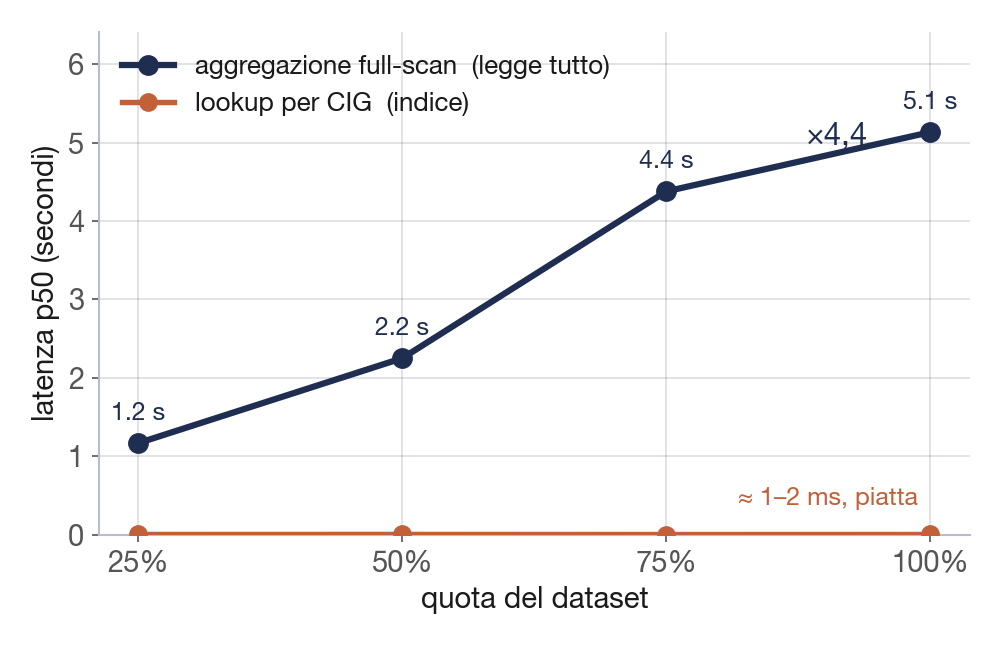
\includegraphics[width=0.66\textwidth]{../../benchmarks/scale-data.png}
\caption{Latenza al crescere del dataset, su un nodo. La query su indice (lookup per CIG)
resta piatta; l'aggregazione full-scan cresce quasi lineare, $\times 4{,}4$ dal 25 al 100\%.}
\label{fig:scale-data}
\end{figure}

\subsection{Quando crescono i nodi: lo sharding}

La seconda angolazione ribalta la prospettiva: i dati restano fissi e si fanno crescere i
nodi. Qui entra in gioco lo sharding di MongoDB. Come shard key abbiamo usato l'hash del CIG
con pre-split, così i documenti si distribuiscono in modo uniforme già all'inserimento, senza
migrazioni di chunk a posteriori né documenti orfani.

Un benchmark di sharding è molto sensibile al disco: su hardware condiviso o con uno storage
lento la curva diventa rumorosa e poco affidabile. Per questo l'abbiamo eseguito su un
\textbf{cluster dedicato} (un droplet DigitalOcean con 4 vCPU dedicate e disco NVMe),
caricando 500 mila lotti e portando lo sharding da 1 a 5 nodi. La curva è regolare e monotòna
su entrambi gli assi (Figura~\ref{fig:scale-shard}):

\begin{itemize}
  \item \textbf{L'aggregazione scende del 41\%} (da 1786 a 1051 ms in mediana): distribuire il
        full-scan sugli shard ed eseguirlo in parallelo ne abbatte la latenza, e scende a ogni
        nodo aggiunto.
  \item \textbf{La scrittura sale del 30\%} (da 20,0k a 25,9k doc/s): gli inserimenti si
        ripartiscono su più nodi.
  \item \textbf{Il lookup per CIG resta attorno ai 2 ms} a qualunque numero di shard: la chiave
        per hash distribuisce il carico senza creare punti caldi.
\end{itemize}

\noindent
In breve: più nodi danno più throughput
in scrittura e meno latenza nelle aggregazioni distribuite, e i percentili al 95 restano
vicini alla mediana, senza picchi.

\begin{figure}[H]
\centering
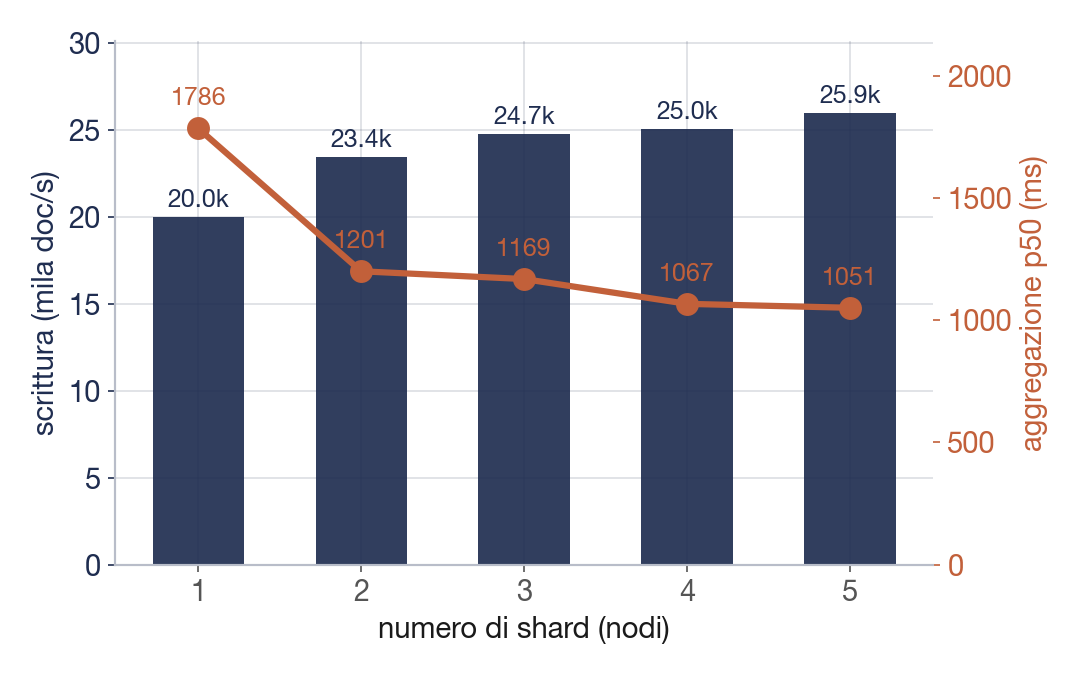
\includegraphics[width=0.72\textwidth]{../../benchmarks/scale-shard.png}
\caption{Sharding da 1 a 5 nodi sul cluster dedicato (4 vCPU, NVMe). Le barre sono il
throughput di scrittura (sale, +30\%), la linea è la latenza dell'aggregazione (scende,
$-41\%$). Curva monotòna su entrambi gli assi.}
\label{fig:scale-shard}
\end{figure}

\noindent
Una precisazione architetturale chiude il quadro, perché distingue ciò che i due database sanno
fare. MongoDB combina due meccanismi: lo \emph{sharding} appena visto, che dà la scala
orizzontale, e il \emph{replica-set}, che dà la disponibilità. Neo4j Community offre solo il
secondo: replica leader/follower per non cadere, ma \emph{non} shardizza il grafo su più nodi.
Non è una svista, ma una proprietà dei due modelli di dato: partizionare un grafo connesso senza
spezzare le relazioni è molto più difficile che partizionare documenti indipendenti per chiave.
La distribuzione \enquote{vera} del carico, da noi, vive quindi su MongoDB; Neo4j si replica
solo per disponibilità.

\subsection{Quando un nodo cade}

Ultima angolazione: il guasto. Replica-set a tre nodi sotto carico continuo e concorrente; a
metà run uccidiamo di colpo il primary con \texttt{docker kill}: un crash vero, non uno
spegnimento ordinato. Cosa succede: gli altri nodi non se ne accorgono subito, ma dopo il
timeout dei battiti (circa 10 secondi, configurabile) eleggono un nuovo primary quasi
all'istante. In quella finestra le scritture restano bloccate; le letture dai secondary non si
fermano mai. Su circa 36.000 scritture solo 16 falliscono davvero (le altre si accodano e
passano alla ripresa) e nessun dato va perso (Figura~\ref{fig:failover}). Uno spegnimento
ordinato (\texttt{docker stop}) farebbe invece uno \emph{step-down} pulito in un secondo: è il
crash non annunciato a costare l'intero timeout di rilevamento.

\begin{figure}[H]
\centering
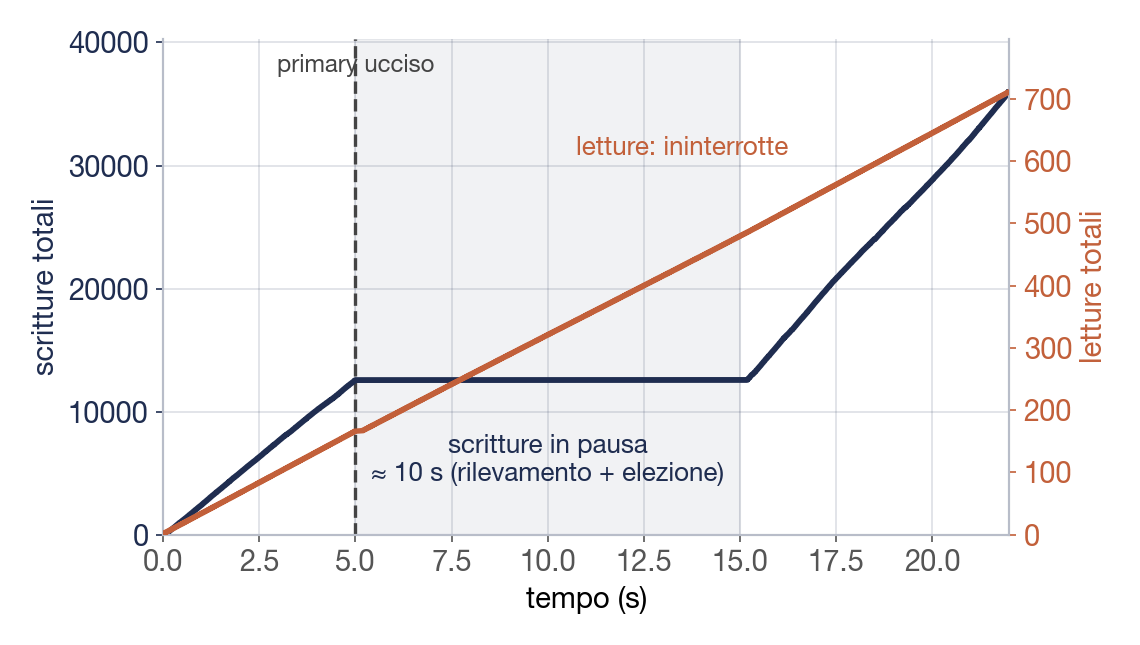
\includegraphics[width=0.74\textwidth]{../../benchmarks/failover-window.png}
\caption{Crollo del primary sotto carico, conteggio cumulativo. La curva delle scritture (navy)
si appiattisce per circa 10 secondi, il tempo di rilevare il guasto ed eleggere un nuovo
primary, poi riprende e recupera la coda accumulata; le letture dai secondary (terracotta)
salgono senza mai interrompersi.}
\label{fig:failover}
\end{figure}

% ====================================================================
\section{Idempotenza dell'ETL}

L'ETL non è un'operazione che si fa una volta sola: i dati ANAC crescono nel tempo, e il
caricamento va ripetuto spesso sul solo delta. La regola che governa tutto è una: rigirare la
pipeline non deve mai creare un doppione. Se ogni riesecuzione reinserisse i documenti già
presenti, i conteggi sarebbero falsati, i benchmark non riproducibili, e il grafo finale pieno
di nodi doppi. Tutto questo poggia su un'unica decisione di progetto (quale campo eleggere a
chiave naturale) che governa insieme l'unificazione delle fonti, la deduplicazione e la
ricostruzione della storia di ogni gara.

\subsection{Due fonti diverse, un record unico}

Le due fonti che alimentano il sistema non condividono né formato né struttura. La Pubblicità
Legale espone gli avvisi nella forma del portale ANAC; l'OCDS segue uno standard
internazionale organizzato per \emph{release}, con una gerarchia di oggetti del tutto diversa.
Ricondurle a una rappresentazione comune è il primo compito della pipeline.

La strada è un modello canonico unico, il \emph{lotto}, verso cui ogni fonte viene tradotta da
un proprio adattatore. L'adattatore della Pubblicità Legale e quello dell'OCDS conoscono la
forma nativa della rispettiva sorgente ed estraggono gli stessi concetti (la gara, le
aggiudicazioni, i contributi, le categorie merceologiche) riversandoli in un'identica
struttura. A valle dell'adattamento, i dati non portano più traccia di dove arrivavano: esiste
un solo tipo di record, qualunque fosse la fonte. È questa normalizzazione preventiva a rendere
possibile l'idea di una chiave unica.

\subsection{Idempotenza a scala piena, e il join fra le fonti}

La prova più diretta dell'idempotenza è rigirare lo stadio \emph{canonical} quando tutti i
grezzi sono già stati consolidati: in quella condizione si ottengono \textbf{0 upsert e 0
duplicati}, a parità di totale complessivo (circa 2,4 milioni di lotti). Non è un caso: i
documenti grezzi usano \texttt{\_id\,=\,idAvviso}, i lotti canonici usano
\texttt{\_id\,=\,CIG}, e si scrive sempre in \emph{upsert}. Riscrivere un documento già
esistente lo aggiorna in posizione invece di duplicarlo; se nulla è cambiato, l'operazione è un
no-op. A protezione del merge, che fonde più documenti sotto lo stesso CIG, ci sono guardie
anti-duplicato su tutte le liste accumulate (avvisi, aggiudicazioni, CPV, rettifiche), così che
nemmeno gli elementi annidati finiscano due volte.

La stessa chiave fa anche un secondo lavoro: il CIG è anche la chiave
di \emph{join} fra le fonti. Lo stesso CIG può comparire sia in Pubblicità Legale sia in OCDS,
con identificativi di documento diversi; ancorando l'identità del lotto al CIG, le due
occorrenze convergono in un solo record canonico invece di restare due voci scollegate. Su un
carico di prova OCDS, dopo il merge \textbf{22.024 lotti} risultano coperti da entrambe le
fonti, e la collezione cresce solo dei lotti realmente inediti, di nuovo l'idempotenza in
azione. Lo stesso meccanismo vale per la storia di una gara: gli atti successivi (nuove
aggiudicazioni, rettifiche, subentri dopo un ricorso) non creano nuovi record, ma si accumulano
sotto lo stesso CIG. Così la catena temporale degli esiti diventa lo \emph{stato} di un singolo
lotto, leggibile in un colpo solo.

\subsection{La stessa impresa, scritta in modi diversi}

C'è un problema gemello, che appartiene allo stesso capitolo: ricomporre l'identità delle
entità. Imprese e stazioni appaltanti compaiono nei dati come \emph{denominazioni testuali}, e
il nome, da solo, non basta a dire quando due record sono lo stesso soggetto. La stessa azienda
può presentarsi con varianti, refusi, abbreviazioni o forme giuridiche diverse, mentre soggetti
distinti possono avere nomi identici. Capire chi è chi, quando manca un identificativo
trasmesso via API, è un problema di \emph{record linkage}.

La prima difficoltà è il numero di confronti. Dai 2,37 milioni di lotti escono 426.564 soggetti
distinti per codice fiscale: confrontare ciascuno con tutti gli altri vorrebbe dire valutare
circa \textbf{91 miliardi} di coppie, una mole impraticabile. La tecnica del \emph{blocking}
serve esattamente a questo, e l'idea è semplice: invece di confrontare ogni impresa con tutte
le altre, si raggruppano i nomi simili in piccoli gruppi (per chiave di nome normalizzato) e si
confrontano solo le coppie \emph{interne} a ciascun gruppo. Le imprese che non finiscono nello
stesso gruppo non vengono nemmeno messe a confronto. L'effetto è drastico: dai 91 miliardi di
coppie potenziali si scende a \textbf{94.100} confronti reali.

Ridurre i confronti non basta, però: per ogni coppia candidata bisogna decidere. E qui la
scelta importante è non fidarsi del nome. Confrontare i soli nomi produce troppi falsi
positivi: due imprese omonime ma distinte verrebbero fuse. La strategia finale àncora quindi
ogni decisione al codice fiscale, usando il nome solo come segnale di candidatura, con quattro
esiti possibili:

\begin{itemize}
  \item \textbf{reject}: due codici fiscali validi e diversi: i soggetti non si collegano,
        per quanto i nomi somiglino;
  \item \textbf{merge}: codice fiscale identico, o chiaramente un refuso dell'altro
        (lo conferma il checksum): si fondono;
  \item \textbf{bridge}: una ditta individuale che compare con la partita IVA in una fonte e
        con il codice fiscale della persona nell'altra: i due identificativi si riconoscono
        come lo stesso soggetto;
  \item \textbf{review}: il nome suggerisce un legame ma il codice fiscale è inconcludente:
        non si forza nulla, la coppia va in una coda di revisione umana.
\end{itemize}

\noindent
Validata su un gold set annotato in modo oggettivo (a partire dal codice fiscale, non dai nomi),
questa strategia raggiunge \textbf{precisione 1,00}. La recall non è perfetta, ed è una scelta
voluta: le coppie \enquote{perse} sono quelle giustamente mandate in revisione, non veri
collegamenti mancati. Il motivo è che questi link alimentano segnalazioni di anomalia, e in
quel contesto un falso positivo, accusare di concentrazione sospetta due imprese che in realtà
sono soggetti distinti, costa molto più di un collegamento in meno.

% ====================================================================
\section{Ricerca vettoriale}

Costruito il sistema, restano da misurare le due componenti con cui lo si interroga. La prima
è la ricerca semantica.

\subsection{Il vantaggio: cercare per significato}

La ricerca classica, per parole chiave, trova un bando solo se contiene esattamente i termini
cercati: chi cerca \enquote{manutenzione del verde} si perde un avviso che parla di
\enquote{sfalcio e potatura}, anche se è la stessa cosa. La ricerca vettoriale serve proprio a
questo. A ogni lotto associamo un \emph{embedding}, un vettore che ne cattura il significato:
bandi che parlano di cose simili finiscono vicini nello spazio, anche quando usano parole
diverse. Cercare diventa allora trovare i vettori più vicini a quello della domanda. Il
vantaggio concreto è una ricerca per \emph{senso} invece che per stringa, ed è ciò che permette
all'agente del capitolo seguente di rispondere a richieste come \enquote{trova gare di pulizia
industriale} senza dipendere dalle parole esatte scritte nei documenti.

Ottenuto questo, resta una domanda di progetto: \emph{dove} conviene calcolare la similarità.
Le due strade sono calcolarla dentro MongoDB, attraversando tutta la collezione, oppure
delegarla a un indice specializzato come quello di Elasticsearch. La risposta è un compromesso,
ed è bene dichiararlo.

\subsection{Forza bruta o indice: MongoDB contro Elasticsearch}

La valutazione usa vettori \emph{reali} a 512 dimensioni (ottenuti per troncamento Matryoshka
dai 1536 originali) e fa variare la scala del corpus su quattro punti, da 125 a 500 mila lotti,
per osservare non un singolo valore ma l'andamento, che è ciò che davvero distingue le due
strategie.

\begin{itemize}
  \item \textbf{MongoDB a forza bruta} confronta la query con tutti i vettori, uno per uno. È
        \emph{esatto al 100\%} e non richiede nessuna infrastruttura oltre a MongoDB. Ma il
        costo è lineare in $N$: la latenza raddoppia a ogni raddoppio del corpus, e a 500 mila
        lotti è già a 183 ms. Estrapolando ai 2,4 milioni di lotti dell'intero dataset si
        arriverebbe attorno agli 880 ms per query, incompatibile con un uso interattivo.
  \item \textbf{Elasticsearch con indice HNSW} non visita tutto il corpus: naviga un grafo di
        prossimità. La latenza cresce in modo nettamente sublineare, ed è già 2,7$\times$ più
        veloce a 125k, con il vantaggio che si \emph{allarga} con la scala fino a 4-5$\times$.
        Il prezzo è duplice: l'indice è approssimato, e il recall@10 scende dal 97,0\% di 125k
        all'89,3\% di 500k; e va costruito e mantenuto, con un costo che cresce coi dati.
\end{itemize}

\subsection{Velocità, throughput ed esattezza}

La differenza si vede su due assi, ed è quello che la Figura~\ref{fig:search} mette a confronto.
Sulla \emph{latenza}, la curva di MongoDB sale lineare mentre quella di Elasticsearch resta
quasi piatta, e la forbice fra le due si allarga con la scala. Sul \emph{throughput}, cioè
quante query al secondo regge ciascun motore, il divario è altrettanto netto: a 500 mila lotti
MongoDB scende a circa 5 query al secondo, mentre Elasticsearch ne sostiene 18; a 125 mila erano
22 contro 30. In un uso con più utenti in parallelo è proprio il throughput a fare la
differenza.

\begin{figure}[H]
\centering
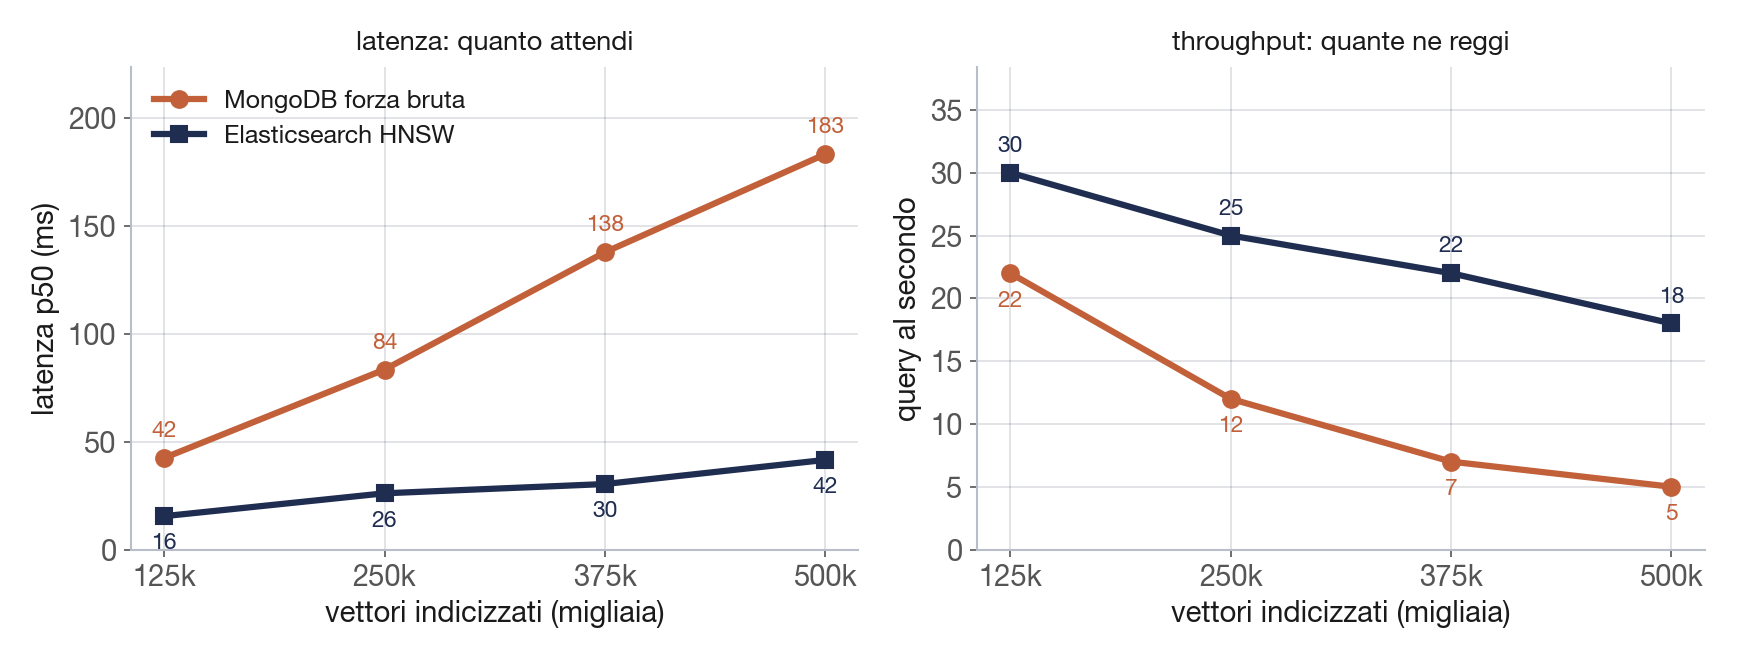
\includegraphics[width=\textwidth]{../../benchmarks/search-tradeoff.png}
\caption{MongoDB a forza bruta contro Elasticsearch (HNSW) al crescere del corpus. A sinistra la
latenza p50 (MongoDB sale lineare, Elasticsearch resta quasi piatto); a destra il throughput in
query al secondo (MongoDB crolla, Elasticsearch regge). La forbice si allarga con la scala.}
\label{fig:search}
\end{figure}

\noindent
Il compromesso, allora, è fra velocità e scala da una parte (Elasticsearch) ed esattezza e
semplicità dall'altra (MongoDB). Sotto circa 100 mila lotti il brute-force basta, ed è
preferibile proprio perché è esatto e non ha niente da gestire. Oltre i 250-500 mila, e
soprattutto per un uso interattivo, Elasticsearch prevale in latenza e in throughput e diventa
la scelta obbligata, accettando in modo consapevole un recall sotto il 100\% come prezzo
dell'approssimazione. Non è una decisione da prendere una volta per tutte, ma in funzione della
scala e di quanto l'applicazione tollera un risultato approssimato.

% ====================================================================
\section{Un agente che interroga i dati}

L'ultimo pezzo è il livello che rende tutto interrogabile parlando. Non è un semplice
traduttore da testo a query, ma un \textbf{agente function-calling} (modello \texttt{gpt-5-mini})
che ragiona a più passi: a ogni turno sceglie uno strumento, ne osserva il risultato e decide
la mossa successiva, fino a un massimo di dieci passi prima di rispondere. La cosa importante è
\emph{dove} sono i suoi strumenti: sono distribuiti sui tre database dell'architettura
poliglotta. È qui che la scelta di tre store specializzati ripaga davvero: l'agente non è
legato a un solo database, ma manda ogni sotto-domanda al motore più adatto a risponderle.

\subsection{Dieci strumenti sui tre store}

La Tabella~\ref{tab:tools} elenca i dieci strumenti, raggruppati per store. La suddivisione
rispecchia l'architettura: il grafo per le relazioni, Elasticsearch per il significato, MongoDB
per il documento canonico, più un paio di strumenti accessori.

\begin{table}[H]
\centering
\footnotesize
\begin{tabular}{@{}llp{7.4cm}@{}}
\toprule
\textbf{Store} & \textbf{Strumento} & \textbf{Cosa fa}\\
\midrule
\multirow{5}{*}{Neo4j}
 & \texttt{risolviEntita}   & risolve un nome impreciso nei candidati reali (full-text fuzzy)\\
 & \texttt{queryGrafo}      & esegue Cypher in sola lettura (conteggi, classifiche, relazioni)\\
 & \texttt{schemaGrafo}     & espone lo schema vivo del grafo\\
 & \texttt{reteEntita}      & rete ego di un'entità, resa come grafo navigabile\\
 & \texttt{metriche}        & aggregazione resa come grafico (barre / linee / torta)\\
\midrule
\multirow{2}{*}{Elasticsearch}
 & \texttt{ricercaSemantica}& ricerca dei bandi per significato (kNN sugli embedding)\\
 & \texttt{gareTema}        & conteggio e classifica delle gare per tema semantico\\
\midrule
MongoDB
 & \texttt{dettaglioBando}  & scheda canonica completa di un CIG\\
\midrule
\multirow{2}{*}{Derivati / esterni}
 & \texttt{stimaPrezzo}     & prezzo di aggiudicazione atteso (kNN su ES + distribuzione dei ribassi)\\
 & \texttt{cercaWeb}        & ricerca web, solo per contesto esterno ai dati ANAC\\
\bottomrule
\end{tabular}
\caption{I dieci strumenti dell'agente, instradati verso lo store più adatto.}
\label{tab:tools}
\end{table}

\subsection{Una domanda, lo store giusto}

Il valore dell'agente non sta nel singolo strumento, ma nel fatto che li orchestra. Una domanda
come \enquote{chi sono i concorrenti di questa impresa} diventa un giro sul grafo; \enquote{trova
i bandi che parlano di X} va a Elasticsearch; \enquote{quanto verrà aggiudicata questa gara}
combina una ricerca semantica con la distribuzione dei ribassi storici. Alcuni strumenti non
restituiscono solo dati ma costruiscono un artefatto: \texttt{metriche} accompagna
un'aggregazione con un grafico, \texttt{reteEntita} restituisce la rete di un'entità come grafo
da esplorare. L'utente chiede in italiano; l'agente sceglie da solo dove e come cercare.

Uno degli strumenti (\texttt{risolviEntita}) risolve i nomi imprecisi nelle entità esatte del
grafo, così l'agente interroga per chiave invece di indovinare con un filtro testuale. Su un
piccolo set di domande di prova, validate a mano, le risposte sono tutte corrette.

% ====================================================================
\section{Conclusioni}

TenLens nasce per mostrare quattro proprietà di un'architettura dati su appalti pubblici reali,
e ognuna è stata chiusa con una misura, non con un'affermazione a parole.

\begin{itemize}
  \item \textbf{Scalabilità.} Due regimi distinti: le query su indice restano logaritmiche e
        quasi insensibili alla mole, mentre le aggregazioni full-scan crescono lineari, ed è
        lì che interviene lo sharding, distribuendo il lavoro sui nodi. Sul cluster dedicato la
        curva da 1 a 5 nodi è regolare su entrambi gli assi; e a un crash del primary reagisce
        da solo, eleggendo un nuovo nodo senza perdere dati: le scritture si fermano per la
        finestra di failover, le letture no.
  \item \textbf{Idempotenza.} Zero duplicati su una riesecuzione completa, grazie al CIG come
        chiave naturale; la stessa chiave fa da join fra Pubblicità Legale e OCDS e accumula la
        storia di ogni gara. Allo stesso capitolo appartiene la ricomposizione delle entità,
        ancorata al codice fiscale.
  \item \textbf{Ricerca vettoriale.} Un compromesso esplicito fra l'esattezza del brute-force di
        MongoDB e la velocità dell'indice HNSW di Elasticsearch, pagata con un po' di recall.
  \item \textbf{L'agente.} Dieci strumenti distribuiti sui tre store, orchestrati da un agente
        che ragiona a più passi: l'architettura poliglotta diventa qualcosa che si interroga in
        italiano.
\end{itemize}

\noindent
Il filo conduttore è uno solo: ogni affermazione ha dietro un numero che la regge, e i limiti
osservati, il recall dell'indice approssimato, la coda di revisione del linkage, sono
dichiarati invece che taciuti.

\end{document}
